\chapter{Conceptual Design}
\label{chap:conceptual-design}
The goal of this thesis is to develop a system that allows generating large sets of images for training neural networks. As this environment shall be used as a drop-in replacement for conventional methods such as taking photos and labelling those by hand, the generated images must be of excellent quality and labelled.\\
This chapter will introduce the terminology, central ideas and architectural basics of a concept that can be used to implement the system by explaining its high-level features using use-cases, refining those to specific user-interactions and deducing components from those. 

%////////////////////////////////////////////////
\section{System Environment and Terminology}
% *** Scenes
The system features at least one virtual 3D environment (a \emph{scene}) that represents a specific place (either an existing or non-existing place) and a virtual \emph{robot} that operates in said environment. It is used by two groups of users: \emph{designers} and \emph{\ac{AI} engineers}. Figure \ref{fig:use-cases-abstract} shows these groups of users and their high-level and abstract use-cases.
\begin{figure}[t]
    \centering
    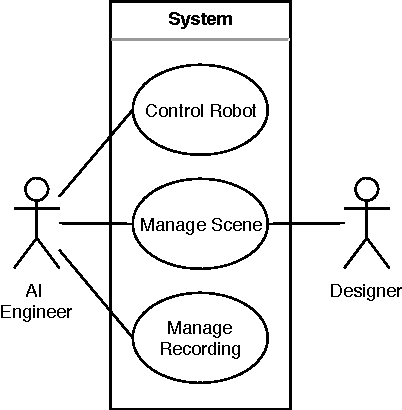
\includegraphics[width=6cm]{img/ch04/UseCases_HighLevel.pdf}
    \captionof{figure}{High-level Use-Cases}
    \label{fig:use-cases-abstract}
\end{figure}
% *** Robots
A \emph{virtual robot} is a representation of a real or fictional robot. It is mainly used to navigate a virtual camera used for capturing \emph{records} from the robot's perspective while its movement is restricted by its body's specifics, considering different types of drives (such as limbs or wheels) and their respective attributes (such as degrees of freedom or torque).\\
% *** Designers
Scenes need to be created, modeled using geometry, populated with entities and configured. \emph{Designers} set up scenes so that they can be used by \acs{AI} engineers in a production environment. They recreate existing or non-existing places by adding 3D objects and \emph{entities} to scenes. Depending on the specific use of the scene and individual objects in it, designers can add \emph{mutators} to any entities in a scene and equip them with an initial configuration. They can also add waypoints to scenes that constitute paths for robots to travel along.\\
% *** Records
A \emph{record} is a data-structure that contains an image and a list of labels. \emph{Labels} hold information about the region in an image that a classifier was identified at. Records may contain meta-data about images, such as the location and view-angles of the camera at the time of capturing the images. This meta-data may prove useful when reconstructing the exact position of robots from generated sets of images. The types asterisked in Figure \ref{fig:classes-record} are placeholders that are implementation-specific.
\begin{figure}[b]
    \centering
    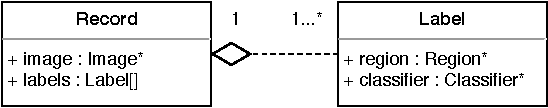
\includegraphics[width=8cm]{img/ch04/Classes_Record.pdf}
    \captionof{figure}{Data-structure "Record"}
    \label{fig:classes-record}
\end{figure}
% *** Entities
\emph{Entities} can be understood as objects in scenes that add more content to a scene than just geometry. Any objects that interact with scenes or other objects within scenes can be understood as entities. This includes light-sources and objects that can be interacted with physically (like doors).
% *** AI engineers
\emph{\acs{AI} engineers} use the system to capture records. To do so they can use the system in one of two modes: \emph{"manual control"} lets them take control of robots and maneuver them in scenes, \emph{"automatic mode"} allows them to let robots travel along preconfigured paths. At any time they can toggle automatic capture and labelling of images and activity of mutators.\\
% *** Mutators
In order to provide visual variety to the generated images, \emph{mutators} alter the state of various attributes of entities in scenes in a step-wise fashion. For instance, they can be used to manipulate the intensity, range and color of light-sources, resulting in images that feature different lighting. The amount of steps a mutator needs to perform alterations on before completing a full mutation-cycle depends on the range of values it can assign to attributes. Binary mutators (e.g. used to turn lights on or off) only take two steps to complete a mutation-cycle, more complex mutators may step through arbitrary value ranges though (e.g. dimming light-intensity from 100 to 0 percent in 5 percent steps, requiring 20 steps total). \\
% *** Waypoints
\emph{Waypoints} (shown in \ref{fig:classes-waypoint}) are simple coordinates in the 3D space of a scene that can be used to define paths that robots can travel along. They may hold a reference to another waypoint, allowing designers and \acs{AI} engineers to easily create paths.  
\begin{figure}[t]
    \centering
    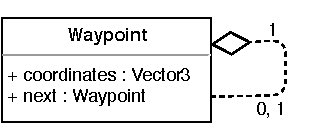
\includegraphics[width=4cm]{img/ch04/Classes_Waypoint.pdf}
    \captionof{figure}{Data-structure "Waypoint"}
    \label{fig:classes-waypoint}
\end{figure}
The specific design of scenes and robots and the implementation of mutators depend on the scenario that the object-recognition software, that is to be trained, is used in: software run on cars should be trained using images generated in scenes that represent the environment the car is planned to be operated in and the robots used in these scenes should be modeled so they closely represent the car the software is to be run on, considering physical attributes (such as the car's shape, surfaces and size), behaviour (including acceleration, weight and steering)  and sensor-placement, where visual sensors such as cameras are of the highest importance to the process of generating images.

%\begin{center}
%\noindent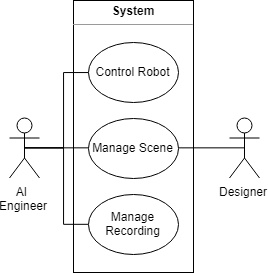
\includegraphics[width=6cm]{img/ch04/Use_Cases_06.png}
%\captionof{figure}{Abstract use-Cases}
%\label{fig:use-cases-abstract}
%\end{center}

%////////////////////////////////////////////////
\section{User Interaction}
The use-cases shown in Figure \ref{fig:use-cases-abstract} need to be further refined into specific features before specific components can be deduced from them.

\subsubsection{Use-Case "Control Robot"}
\acs{AI} engineers may want to take control of robots and maneuver them in scenes by accelerating, decelerating and steering or resetting them in case of being unable to maneuver. This may be the case when the robot was flipped or trapped between objects. Operating in manual mode can also be used to evaluate the usefulness (e.g. mobility) of certain robot-bodies in certain environments, presuming that the scene and robot behave like they would in real-life, and may even be used to validate that the specific combination of robot-body and scene in a scenario operates as expected. This may require physics simulation for gravity and collision detection, and mechanics simulation for kinematics.\\
Also, manual control of robots requires a careful choice of input-devices: \acs{AI} engineers should use input-devices that allow for precise and true to original control of robots. For instance, a combination of a steering wheel and gas and break pedals closely resembles the control options present in cars whereas two independent joysticks can be used to control torque of two continuous tracks on tracked vehicles.

\subsubsection{Use-Case "Manage Recording"}
\acs{AI} engineers need to be able to start and stop automatic capturing of records. As records are effectively pairs of images and a list of labels, both elements of these pairs must be provided by the system: it needs to feature a component that captures images from a camera held by a robot in a scene. To populate records with labels the system needs to provide a component that identifies classifiers in the captured images.

\subsubsection{Use-Case "Manage Scene"}
Designers need to import assets (such as 3D models, materials and textures) into the system in order to add geometry to scenes and configure robots that can be used by \acs{AI} engineers. Depending on the requirements of the scenario at hand, designers may need to add various entities such as light-sources or movable objects to scenes and equip them with an initial set of configurable mutators. Optionally, designers may add waypoints to scenes to provide paths for robots to travel along.\\
\acs{AI} engineers may want to configure mutators at run-time in order to explore and study their effects on scenes (such as changes in lighting). Also they may want to add or change waypoints to vary what part of a scene is captured during recording sessions.

Figure \ref{fig:use-cases} summarizes these refinements and shows that most use-cases are interacted with by only one role, separating them into groups of use-cases required for initial setup ("Create ..."), run-time ("Robot" and "Recording" use-cases) and a special group that is used to tweak run-time behaviour to achieve varying sets of records ("Manage Waypoints", "Manage Mutators"). 
\begin{figure}
    \centering
    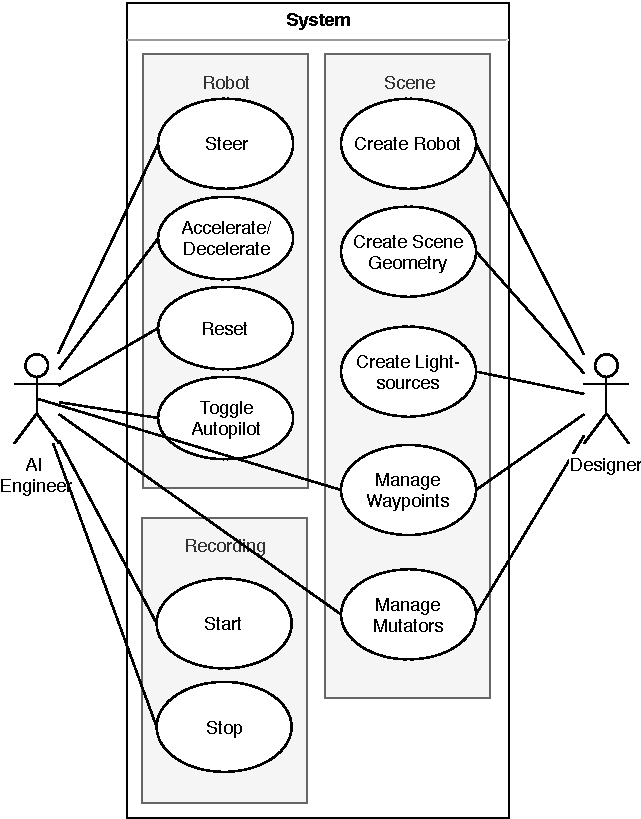
\includegraphics[width=10cm]{img/ch04/UseCases_Fine.pdf}
    \captionof{figure}{Refined Use-Cases}
    \label{fig:use-cases}
\end{figure}
\clearpage

%////////////////////////////////////////////////
\section{Automatic Mode: Control Flow}
\label{ch04-control-flow}
The abovementioned automatic mode the system can run in (shown in Figure \ref{fig:control-flow}) is used to automate the process of moving robots in scenes, capturing records and mutating scenes.\\
When active, it will alter a scene by advancing mutation and capture records as long as the mutation-cycle has not been completed. Once the mutation-cycle is completed, the mutation will be reset. If the robot in the scene has not reached its destination yet it will be moved and the process continues by running the mutation-cycle again.\\
\begin{figure}[htb!]
    \centering
    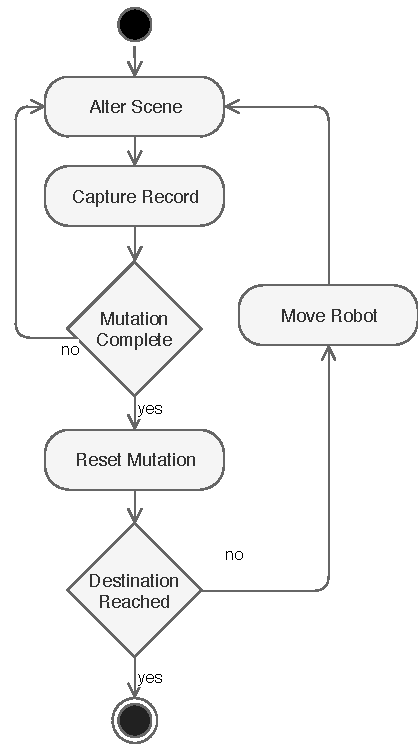
\includegraphics[width=8cm]{img/ch04/ActivityDiagram_HighLevel.pdf}
    \captionof{figure}{Control flow of the automatic mode}
    \label{fig:control-flow}
\end{figure}
This behaviour effectively iterates through all mutations set up for a scene, applies them, captures records for each mutation and does so each time the robots is moved. The only step that is largely independent of implementation is "Reset Mutation" as it will only recover the initial state of all entities in a scene. "Alter Scene", "Capture Record" and "Move Robot" are heavily dependent on the scenario at hand and the specific implementation. For instance, "Move Robot" may either simulate movement of robots by using their physical properties and bodies or simply move them to another position instantly.

%////////////////////////////////////////////////
\section{Components}
While the high-level use-cases (Figure \ref{fig:use-cases-abstract}) implicate the need for three high-level components, refinement of the use-cases (Figure \ref{fig:use-cases}) encourages the use of packages to encapsulate complex components. Figure \ref{fig:component-diagram} shows an abstract component used for controlling robots (\emph{RobotController}), a package that provides components needed for capturing records (\emph{Recording}) and another one that contains components used to manage scenes (\emph{SceneManagement}).
\begin{figure}[hb!]
    \centering
    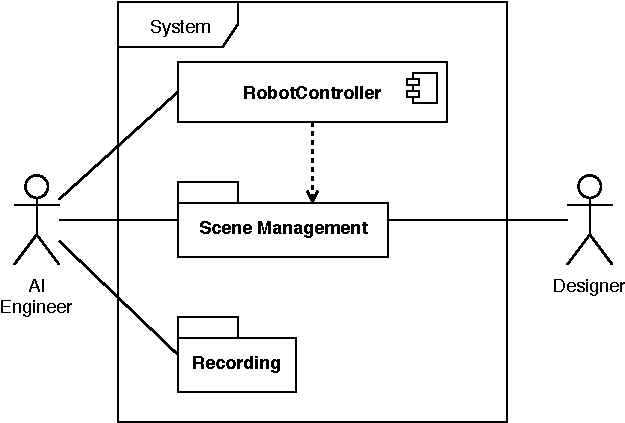
\includegraphics[width=10cm]{img/ch04/ComponentDiagram_System.pdf}
    \captionof{figure}{High-level component diagram}
    \label{fig:component-diagram}
\end{figure}
% Recording
The "Recording"-package (Figure \ref{fig:component-diagram-recording}) contains two abstract components: \emph{CaptureController} is used to start and stop automatic capturing of records. It captures images and enriches those with labels by making use of the \emph{ImageLabeller}-component. The ImageLabeller-component needs to be able to identify classifiers in images. As neither capturing images nor identifying classifiers are necessarily trivial tasks, the implementation of both components is greatly influenced and in some cases dictated by the scenario and technology used. While capturing images is usually easily achieved in software that features visualization of the virtual environments, "headless" software running without any visual output may require external software to render images resulting in the CaptureController-component effectively being implemented by software running on two separate systems, increasing the complexity of the implementation.
\begin{figure}
    \centering
    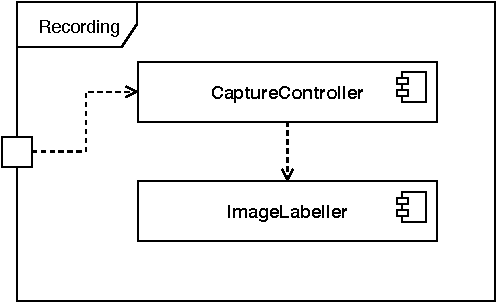
\includegraphics[width=8cm]{img/ch04/ComponentDiagram_Recording.pdf}
    \captionof{figure}{"Recording"-package}
    \label{fig:component-diagram-recording}
\end{figure}
% Scenemanagement
As indicated by the use-cases involved in interacting with scenes (Figure \ref{fig:use-cases}), the "SceneManagement"-package (Figure \ref{fig:component-diagram-scenemanagement}) features multiple components.\\
The \emph{SceneGeometry}-component holds all 3D objects of a scene that amount to the visual representation and physical bodies of the place the scene is meant to represent. This includes both, objects that feature or lack actual physical collision (e.g. clouds).\\
A \emph{SceneEntities}-component stores all entities of a scene and manages their life-cycles. In a simple implementation this component could use lists or arrays internally.
\begin{figure}[hb!]
    \centering
    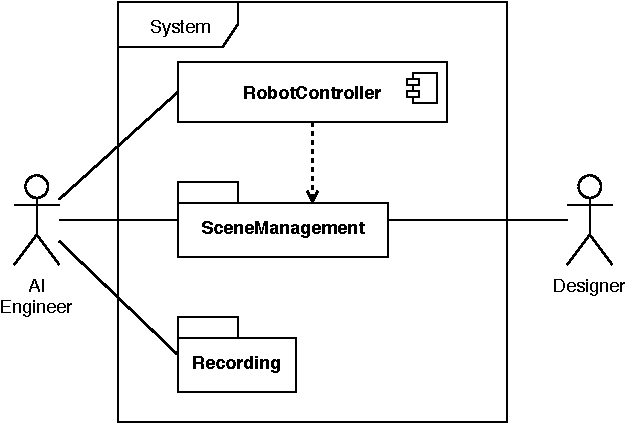
\includegraphics[width=11cm]{img/ch04/ComponentDiagram_SceneManagement02.pdf}
    \captionof{figure}{"SceneManagement"-package}
    \label{fig:component-diagram-scenemanagement}
\end{figure}
In each scene there is one \emph{MutationManager}-component. It holds a list of all mutators in a scene and, when active, advances only one mutator in a scene at a time so that each possible combination of attribute-mutations is present in a scene at least once. This implicates that each additional mutator added to a scene multiplies the number of steps required to fully step through all attribute-mutations by the number of steps required to step through the new mutator; the number of mutation-steps required to complete a full mutation-cycle grows exponentially.\\
The MutationManager-component also provides a reset-feature that resets all attribute-mutations to a defined initial state.
The \emph{WaypointManager}-component holds a list of waypoints where each waypoint constitutes a path by chaining references to other waypoints. Its purpose is to provide an overview of paths configured in scenes.
%
%\section{Summary}
%This concept is designed so that it is operating-system-, platform- and framework-agnostic. This results in an abstract concept that describes a basic architecture and abstract components and allows for flexibility in implementations: components may be implemented and run on the same or many separate machines, which is of particular interest for research-facilities that operate large clusters of computers.